%%%%%%%% ICML 2026 two-column format, [preprint] mode for arXiv %%%%%%%%
% Same template as tomkimpson/power-to-flops (paper/main.tex at 66f6f95). Style
% files are verbatim from that repo.

\documentclass{article}

\usepackage{microtype}
\usepackage{graphicx}
\usepackage{booktabs}
\usepackage{array}
\usepackage{placeins}  % \FloatBarrier: appendix floats stay in their section
\graphicspath{{../figures/}}

% hyperref makes hyperlinks in the resulting PDF.
\usepackage{hyperref}

% Attempt to make hyperref and algorithmic work together better:
\newcommand{\theHalgorithm}{\arabic{algorithm}}

% [preprint] shows authors and drops the review-mode footer — arXiv version.
% Swap to plain \usepackage{icml2026} for a blind submission, or
% \usepackage[accepted]{icml2026} for camera-ready.
\usepackage[preprint]{icml2026}
\captionsetup[table]{position=below}  % table captions sit under their tables

\usepackage{amsmath}
\usepackage{amssymb}
\usepackage{amsfonts}
\usepackage{nicefrac}
\usepackage[capitalize,noabbrev]{cleveref}
\usepackage{subcaption}

% Let page-wide floats take most of a page, so the tall F1 does not queue the rest.
\renewcommand{\dbltopfraction}{0.95}
\renewcommand{\dblfloatpagefraction}{0.8}
% Let column floats sit above text rather than alone in a centred float column.
\renewcommand{\topfraction}{0.9}
\renewcommand{\bottomfraction}{0.8}
\renewcommand{\textfraction}{0.15}
\renewcommand{\floatpagefraction}{0.8}
\usepackage{dblfloatfix}

% generated by scripts/paper_numbers.py from paper/numbers.toml; do not edit by hand
\newcommand{\Ztwo}{100}  % results/heldout/h2.json:headline.Z_r1.detection
\newcommand{\Xprime}{100}  % results/heldout/h2.json:headline.X_prime_classifier.detection
\newcommand{\TauRone}{0.629}  % results/heldout/thresholds.json:r1.threshold
\newcommand{\TauClf}{0.0}  % results/heldout/thresholds.json:classifier.fits.co-location.threshold
\newcommand{\FprRoneDecode}{0.6}  % results/heldout/h2.json:headline.r1_test_fpr.serving-decode
\newcommand{\FprRoneIdle}{0.1}  % results/heldout/h2.json:headline.r1_test_fpr.idle
\newcommand{\ExpDecodeH}{0.475}  % results/monitor/false_alarms.json:backgrounds.declared inference.r1.exposure_h
\newcommand{\FRoneDecode}{0.0}  % results/monitor/false_alarms.json:backgrounds.declared inference.r1.F_per_h
\newcommand{\FupRoneDecode}{6.3}  % results/monitor/false_alarms.json:backgrounds.declared inference.r1.F_upper95_poisson_model
\newcommand{\FClfDecode}{6.3}  % results/monitor/false_alarms.json:backgrounds.declared inference.classifier.F_per_h
\newcommand{\AClfDecode}{0.010}  % results/monitor/false_alarms.json:backgrounds.declared inference.classifier.A
\newcommand{\ARoneBusy}{0.998}  % results/monitor/false_alarms.json:backgrounds.non-AI busy.r1.A
\newcommand{\EpDelayRone}{3.0}  % results/monitor/episodes.json:detectors.r1.pooled_median_delay_s
\newcommand{\LminRone}{5.1}  % results/monitor/episodes.json:detectors.r1.Lmin_s
\newcommand{\GkHardPrefill}{100}  % results/gk/t5.json:forests.hardened.gate_inference.by_condition.serving-prefill.flag_rate
\newcommand{\GkGenPrefill}{2.4}  % results/gk/t5.json:forests.genuine.gate_inference.by_condition.serving-prefill.flag_rate
\newcommand{\GkGenMiss}{0}  % results/gk/t5.json:forests.genuine.co-location.per_run.panel-mixture-concurrent-0p5.detection
\newcommand{\GPU}{H200 NVL}  % paper/setup.json:gpu.name
\newcommand{\Probe}{Micsig RCP120}  % paper/setup.json:probe.model
\newcommand{\ProbeSens}{50}  % paper/setup.json:probe.sensitivity_mV_per_A
\newcommand{\ProbeLo}{34}  % paper/setup.json:probe.band_lo_hz
\newcommand{\ProbeHi}{30}  % paper/setup.json:probe.band_hi_mhz
\newcommand{\Fs}{199,808}  % paper/setup.json:sample_rate_sps
\newcommand{\EnvFrame}{2}  % paper/setup.json:envelope_frame_ms
\newcommand{\ModelParams}{168}  % paper/setup.json:model.params_millions
\newcommand{\PosControlMin}{99}  % paper/setup.json:r1_positive_control_min_pct
\newcommand{\ModelLayers}{8}  % paper/setup.json:model.n_layer
\newcommand{\ModelWidth}{1024}  % paper/setup.json:model.d_model
\newcommand{\RhoLo}{0.25}  % paper/setup.json:colocation_share.low
\newcommand{\RhoMid}{0.5}  % paper/setup.json:colocation_share.mid
\newcommand{\RhoHi}{0.75}  % paper/setup.json:colocation_share.high
\newcommand{\DefaultDecision}{0.5}  % paper/setup.json:default_decision
\newcommand{\GkNFeat}{30}  % paper/setup.json:gk.n_features
\newcommand{\GkRate}{9.765625}  % paper/setup.json:gk.rate_msps
\newcommand{\GkRateApprox}{10}  % paper/setup.json:gk.rate_msps
\newcommand{\GkDecimated}{200}  % paper/setup.json:gk.decimated_ksps
\newcommand{\GkFone}{0.955}  % paper/setup.json:gk.macro_f1
\newcommand{\GkAcc}{0.97}  % paper/setup.json:gk.accuracy
\newcommand{\GkAliasKhz}{10}  % paper/setup.json:gk.alias_khz
\newcommand{\NCaptures}{62}  % results/windows/manifest.json:n_captures
\newcommand{\CorpusHours}{23.4}  % results/windows/manifest.json:captures
\newcommand{\Win}{5}  % results/windows/manifest.json:window_s
\newcommand{\HopSnap}{5}  % results/windows/manifest.json:hops_s.0
\newcommand{\HopMon}{1}  % results/windows/manifest.json:hops_s.1
\newcommand{\CorpusCommit}{73ffebe}  % results/windows/manifest.json:corpus_commit
\newcommand{\NFeat}{25}  % results/replication/t3.json:n_features
\newcommand{\NRepTraces}{300}  % results/replication/t3.json:n_traces
\newcommand{\SoneFone}{0.933}  % results/replication/t3.json:two_stage.macro_f1
\newcommand{\Alpha}{0.05}  % results/heldout/h2.json:alpha
\newcommand{\FracCalZero}{98.8}  % results/heldout/thresholds.json:classifier.fits.co-location.frac_calibration_zero
\newcommand{\RoneMinGroup}{99.9}  % results/heldout/h2.json:r1.detection
\newcommand{\ClfJitterWorst}{76}  % results/heldout/h2.json:classifier.jitter.detection.all.per_run
\newcommand{\GateTrain}{80}  % results/gk/t5.json:forests.hardened.gate.training_min
\newcommand{\GateInf}{20}  % results/gk/t5.json:forests.hardened.gate.inference_max
\newcommand{\Rearm}{5}  % results/monitor/false_alarms.json:rule.rearm
\newcommand{\ExpIdleH}{8.35}  % results/monitor/false_alarms.json:backgrounds.idle.r1.exposure_h
\newcommand{\ExpDeclH}{8.8}  % results/monitor/false_alarms.json:backgrounds
\newcommand{\OnsetsRoneDecl}{1}  % results/monitor/false_alarms.json:backgrounds
\newcommand{\EpTotal}{192}  % results/monitor/episodes.json:detectors.r1.cells
\newcommand{\EpMinDur}{5.1}  % results/monitor/episodes.json:detectors.r1.cells
\newcommand{\EpMaxDur}{240}  % results/monitor/episodes.json:detectors.r1.cells
\newcommand{\Grace}{5}  % results/monitor/episodes.json:rule.grace_s
\newcommand{\EpTruncated}{4}  % results/monitor/episodes.json:detectors.r1.counts.truncated
\newcommand{\EpScored}{188}  % results/monitor/episodes.json:detectors.r1.cells
\newcommand{\LminLevel}{0.5}  % results/monitor/episodes.json:rule.lmin_level
\newcommand{\TfourMisCoPooled}{0}  % results/robustness/t4.json:misspecified_declaration.pooled.h2.r1.co-location.pooled
\newcommand{\TfourMisCoDeclared}{100}  % results/robustness/t4.json:misspecified_declaration.declared.h2.r1.co-location.pooled
\newcommand{\GkNTraces}{1610}  % results/gk/t5.json:forests.hardened.n_fit_traces
\newcommand{\GkOwnFone}{0.891}  % results/gk/t5.json:own_check.macro_f1_mean
\newcommand{\GkOwnFoneLo}{0.845}  % results/gk/t5.json:own_check.macro_f1_range.0
\newcommand{\GkOwnFoneHi}{0.945}  % results/gk/t5.json:own_check.macro_f1_range.1
\newcommand{\GkOwnAcc}{0.908}  % results/gk/t5.json:own_check.accuracy_mean
\newcommand{\GkShuffle}{0.306}  % results/gk/t5.json:own_check.negative_control.macro_f1
\newcommand{\GapGuard}{0.2}  % results/monitor/episodes.json:rule.gap_guard
\newcommand{\ARoneDecode}{0}  % results/monitor/false_alarms.json:backgrounds.declared inference.r1.A
\newcommand{\XzeroPrime}{0.6}  % results/heldout/operating_point.json:replica.tau_alpha.detection_per_run.panel-mixture-concurrent-0p5
\newcommand{\RepPrefill}{100}  % results/heldout/operating_point.json:replica.tau_alpha.fpr.development.serving-prefill
\newcommand{\ClfDevPrefill}{4}  % results/heldout/operating_point.json:classifier.tau_alpha.fpr.development.serving-prefill
\newcommand{\EpPreRone}{47}  % results/monitor/episodes.json:detectors.r1.counts.pre-alarmed
\newcommand{\GkTraceS}{5}  % paper/setup.json:gk.trace_s
\newcommand{\RtWinLo}{5}  % paper/setup.json:rt_window_s.0
\newcommand{\RtWinHi}{60}  % paper/setup.json:rt_window_s.1
\newcommand{\ChainBelowBand}{99.3}  % paper/setup.json:chain_check.train_var_frac_below_20khz
\newcommand{\ChainBandKhz}{20}  % paper/setup.json:chain_check.band_khz
\newcommand{\ChainEnvPct}{0.3}  % paper/setup.json:chain_check.envelope_match_pct_vs_2msps
\newcommand{\FupClfDecode}{16.3}  % results/monitor/false_alarms.json:backgrounds.declared inference.classifier.F_upper95_poisson_model
\newcommand{\RonePrefillHoldout}{100}  % results/declaration/heldout.json:results.6.check4.per_run.panel-serving-prefill.fp_rate
\newcommand{\TauDecOnlyPooled}{0.786}  % results/heldout/r1_scores.json:thresholds.decode_only.pooled calibration
\newcommand{\TauDecOnlyDecode}{0.569}  % results/heldout/r1_scores.json:thresholds.decode_only.decode calibration
\newcommand{\RoneAucDecode}{0.994}  % figures/f7_r1.json:annotated.r1.auc_unpaced_vs_test_decode
\newcommand{\RoneDecodeAboveMin}{0.6}  % figures/f7_r1.json:annotated.r1.frac_test_decode_above_unpaced_min
\newcommand{\RoneCalIdle}{9}  % results/declaration/heldout.json:results.6.cal_fp_by_workload.idle
\newcommand{\Digitiser}{PicoScope 5464E}  % paper/setup.json:digitiser.model
\newcommand{\DigBits}{16}  % paper/setup.json:digitiser.bits
\newcommand{\BurstRate}{100}  % paper/setup.json:aliasing.burst_rate_msps
\newcommand{\AliasTrainPct}{0.32}  % paper/setup.json:aliasing.train_folded_pct
\newcommand{\AliasIdleX}{13}  % paper/setup.json:aliasing.idle_folded_ratio
\newcommand{\BootBlock}{12}  % paper/setup.json:intervals.block_windows
\newcommand{\BootBlockS}{60}  % paper/setup.json:intervals.block_s
\newcommand{\NBoot}{2,000}  % paper/setup.json:intervals.n_boot
\newcommand{\EpBlock}{4}  % paper/setup.json:intervals.episode_block
\newcommand{\OnsetBlockMin}{10}  % paper/setup.json:intervals.onset_block_min
\newcommand{\TfourIdleADecode}{99.97}  % results/robustness/t4.json:misspecified_declaration.declared.h3.r1.false_alarms.idle.A
\newcommand{\NBootBound}{10,000}  % paper/setup.json:intervals.n_boot_bound
\newcommand{\ForestTrees}{500}  % paper/setup.json:forest_trees
\newcommand{\TauRoneLo}{0.545}  % results/heldout/thresholds.json:r1.stability.ci95.0
\newcommand{\TauRoneHi}{0.641}  % results/heldout/thresholds.json:r1.stability.ci95.1
\newcommand{\AlphaPct}{5}  % results/heldout/h2.json:alpha
\newcommand{\EthreeKOne}{4}  % results/heldout/e3_calibration_breakdown.json:breakdown_by_alpha.0.01.n_windows
\newcommand{\EthreeKFive}{18}  % results/heldout/e3_calibration_breakdown.json:breakdown_by_alpha.0.05.n_windows
\newcommand{\EthreeKTen}{38}  % results/heldout/e3_calibration_breakdown.json:breakdown_by_alpha.0.1.n_windows
\newcommand{\EthreeCalWindows}{340}  % results/heldout/e3_calibration_breakdown.json:calibration_windows
\newcommand{\EthreeHonestMin}{99.66}  % results/heldout/e3_calibration_breakdown.json:breakdown_honest_min
\newcommand{\DecodeRuns}{5}  % results/heldout/e3_calibration_breakdown.json:decode_summary.n_runs
\newcommand{\DecodeSessions}{4}  % results/heldout/e3_calibration_breakdown.json:decode_summary.n_sessions
\newcommand{\DecodeWindows}{850}  % results/heldout/e3_calibration_breakdown.json:decode_summary.n_windows
\newcommand{\DecodeFlagged}{5}  % results/heldout/e3_calibration_breakdown.json:decode_summary.n_flagged
\newcommand{\PrefillInFitFlagged}{1}  % results/heldout/e3_calibration_breakdown.json:dev_prefill_in_fit.n_flagged
\newcommand{\PrefillInFitN}{170}  % results/heldout/e3_calibration_breakdown.json:dev_prefill_in_fit.n
\newcommand{\RoneUnpacedMin}{0.658}  % results/heldout/e3_calibration_breakdown.json:unpaced_margin.run_min
\newcommand{\RoneMargin}{0.017}  % results/heldout/e3_calibration_breakdown.json:unpaced_margin.margin_over_tau_ci95_hi
\newcommand{\DeclBandLo}{0.39}  % results/heldout/e3_calibration_breakdown.json:score_band_min_median_max.full
\newcommand{\DeclBandHi}{0.68}  % results/heldout/e3_calibration_breakdown.json:score_band_min_median_max.full
\newcommand{\HidBandLo}{0.66}  % results/heldout/e3_calibration_breakdown.json:score_band_min_median_max.full
\newcommand{\HidBandHi}{0.71}  % results/heldout/e3_calibration_breakdown.json:score_band_min_median_max.full
\newcommand{\EfourKHonest}{50}  % results/heldout/e4_fit_contamination.json:grid.6.k
\newcommand{\EfourShareHonest}{7}  % results/heldout/e4_fit_contamination.json:grid.6.share_of_fit
\newcommand{\EfourFullCal}{0}  % results/heldout/e4_fit_contamination.json:grid.6.calibration_honest_by_run.panel-core-training-r4.median
\newcommand{\EfourLoraCal}{100}  % results/heldout/e4_fit_contamination.json:grid.6.calibration_honest_by_run.panel-core-lora-r4.median
\newcommand{\EfourKHalf}{500}  % results/heldout/e4_fit_contamination.json:smallest_k.0.5.k
\newcommand{\EfourKGone}{1000}  % results/heldout/e4_fit_contamination.json:smallest_k.0.05.k
\newcommand{\EfourShareGone}{60}  % results/heldout/e4_fit_contamination.json:smallest_k.0.05.share_of_fit
\newcommand{\EfourNDraws}{20}  % results/heldout/e4_fit_contamination.json:grid.6.n_draws
\newcommand{\EfourNDeclared}{680}  % results/heldout/e4_fit_contamination.json:n_declared_fit
\newcommand{\TfourPosCtrl}{0.17}  % results/heldout/e3_calibration_breakdown.json:decode_only_flag_rates.honest training.pooled
\newcommand{\RoneHonestFull}{100}  % results/heldout/e3_calibration_breakdown.json:curve_alpha_0.05.0.rates.honest training
\newcommand{\DecOnlyPrefillPooled}{0}  % results/heldout/e3_calibration_breakdown.json:decode_only_flag_rates.declared development serving-prefill.pooled
\newcommand{\EfourHalfDet}{35}  % results/heldout/e4_fit_contamination.json:grid.9.unpaced_detection.median
\newcommand{\EfourGoneDet}{0}  % results/heldout/e4_fit_contamination.json:grid.10.unpaced_detection.median
\newcommand{\SessSame}{11}  % results/heldout/session_check.json:results.iforest.pooled.S
\newcommand{\SessOther}{29}  % results/heldout/session_check.json:results.iforest.pooled.O
\newcommand{\SessPair}{22}  % results/heldout/session_check.json:results.iforest.per_run.panel-core-serving-decode-r1.other_run_fp_by_run.panel-core-serving-decode-r4
\newcommand{\SessRefWindows}{10}  % results/heldout/session_check.json:design.n_ref
\newcommand{\SessRuns}{3}  % results/heldout/session_check.json:decode_runs
\newcommand{\FeightBin}{0.25}  % results/monitor/traces.json:envelope.bin_s
\newcommand{\RobCoMin}{100}  % results/robustness/t4.json:alpha_sweep
\newcommand{\RobOnDecAlpha}{0}  % results/robustness/t4.json:alpha_sweep
\newcommand{\RobOnIdleAlpha}{4}  % results/robustness/t4.json:alpha_sweep
\newcommand{\RobOnDecPers}{2}  % results/robustness/t4.json:persistence
\newcommand{\RobOnIdlePers}{4}  % results/robustness/t4.json:persistence
\newcommand{\EfourDeclZero}{0.6}  % results/heldout/e4_fit_contamination.json:grid.0.declared_fit_flag_rate.median
\newcommand{\EfourDeclEnd}{0.0}  % results/heldout/e4_fit_contamination.json:grid.-1.declared_fit_flag_rate.median
\newcommand{\AcRmsUnpaced}{10.4}  % results/heldout/ac_rms.json:runs.panel-mixture-concurrent-0p5.median_a
\newcommand{\AcRmsDecode}{5.3}  % results/heldout/ac_rms.json:runs.panel-serving-decode.median_a
  % every number in the prose (scripts/paper_numbers.py)

% Short form of the title for the running header:
\icmltitlerunning{Verifying Declared AI Workloads from GPU Supply Current}

\begin{document}

\twocolumn[
  \icmltitle{Verifying Declared AI Workloads from GPU Supply Current}

  \begin{icmlauthorlist}
    \icmlauthor{Tom Kimpson}{unimelb,mats}
  \end{icmlauthorlist}

  \icmlaffiliation{unimelb}{School of Mathematics and Statistics, The University of Melbourne, Parkville, VIC, Australia}
  \icmlaffiliation{mats}{Machine Alignment, Transparency \& Security (MATS)}

  \icmlcorrespondingauthor{Tom Kimpson}{tom.kimpson@unimelb.edu.au}

  % Keywords populate the PDF metadata; they are not shown in the document.
  \icmlkeywords{AI governance, compute verification, declared workloads, hidden training, side channels, current sensing, anomaly detection, one-class models}

  \vskip 0.3in
]

% Creates the first-column footnote with affiliations; required even if empty.
\printAffiliationsAndNotice{}

\begin{abstract}
An agreement on AI compute needs a way to check that each GPU runs only the work its
operator declares. We show that an external observer can identify departures from the
declared work on one NVIDIA \GPU{} GPU from its supply current alone, with no
examples of hidden training to learn from. We record \CorpusHours{}~h of current with a clamp-on
probe, covering declared work (inference and idle), honest training, and training hidden
by five evasion strategies. A one-class model learns only from recordings of the
declared work, its reference. It flags \Ztwo\% of training that runs beside declared
inference. As a monitor on a held-out day, it detects all \EpScored{} hidden training
episodes, with a median delay of \EpDelayRone{}~s, and raises no alarm in
\ExpDecodeH{}~h of declared inference. The check needs a complete reference. With
idle missing from the reference, the monitor is in alarm for \TfourIdleADecode\% of
declared idle. With idle used only to set the alarm threshold, the monitor misses all
\EpScored{} episodes and raises no alarm on declared inference. Training in the
reference has the same silent effect. These results come from one GPU
and one model. They indicate that a declaration can replace a catalogue of evasions, and
that the security of the check then rests on how the verifier obtains the reference.
\end{abstract}



\section{Introduction}\label{s:intro}

Agreements on AI compute will need a way to check how a GPU is
used~\citep{shavit2023,baker2025}. The operator states the work that a GPU runs, its
\emph{declaration}. The verifier does not trust the declaration, and must check that
the GPU runs nothing else, such as hidden training. \citet{scher2025} describe two ways to use physical measures of chip activity, such as power draw, to perform this check. In their
\emph{default approach}, the verifier fits a classifier on many workloads that it labels and
runs on its own chips, then applies it to the operator's chips. Such a classifier must transfer from the chips it
was fitted on to the chips it monitors. In their alternative approach, the verifier's inspectors,
with temporary access to the operator's code, confirm that the chips run only the declared
work and record their activity while they do. This recording is a signature of the work. Later, the verifier
monitors the chips' activity and investigates when it departs from the
signatures~\citep{scher2025}. We call this a \emph{signature check}. It needs no transfer between chips, and it is harder to
evade, because the operator's chips must look like the declared work, not merely unlike
training~\citep{scher2025}. A related
proposal counts the chip-hours whose signature matches a verified workload, with
signatures taken from the verifier's own hardware or from a model of the
workload~\citep{baker2025}.

Existing empirical studies of hidden training have focused on the default approach.
\citet{gargiulo2026}
measure the current drawn by a GPU. A random forest fitted to these traces tells
training from inference and non-AI work with 97\% accuracy on model families it has
not seen. \citet{rahman2026} reach 98\% from sliding windows of on-chip telemetry
across nine GPU types. Both studies test their classifiers against operators who try to
hide training. Detection stays high against most evasions but falls against some that
the classifiers were not fitted to: to 43\% for white-box diluted low-rank adaptation in
\citet{rahman2026}, and to 48--88\% for diluted low-rank adaptation in
\citet{gargiulo2026}. A second test in \citet{gargiulo2026}, which flags the
brief dip in current left by each optimizer update, raises detection of diluted low-rank
adaptation to at least 98\%.

We found no empirical study of how well a signature check works. Power signatures do
identify workloads on high-performance computing systems~\citep{copos2020,kohler2021,karimi2024},
but those studies assume an operator who does not try to hide work~\citep{scher2025}. \citet{scher2025} name several uncertainties
in the signature check, among them which chip activity to measure, how stable signatures
stay over time, how often inspectors can investigate an alarm, how finely to define
workloads, and whether the chip activity of each workload is specific enough to tell it apart.
Unlike the default approach, the signature check uses the operator's declaration, because
its signatures are recordings of the declared work. Declared work has helped
in related settings. A bound on hidden compute from power draw tightens sharply once the
verifier can re-run the declared work \citep{kimpson2026}. In simulated datacentre power
traces, a tracker with its threshold set on declared work detects at least 96\% of training
runs hidden in declared inference, at a 1\% false-alarm rate \citep{kimpson2026datacentre}.

In this work we test the signature check on one \GPU{}. A current probe owned by the
verifier is clamped to the GPU's auxiliary supply and records \CorpusHours{}~h of current
(\cref{s:setting}). We record declared work
(serving decode, serving prefill and idle), honest training, and several evasion
strategies, in particular \emph{co-location}: training runs as a second process beside
the declared inference and uses the capacity that inference leaves spare. We fit
classifiers to labelled examples of training to stand for the default approach. Our signature
check is a one-class model fitted only to recordings of the declared work, with its threshold set
on separate recordings of that work, so it needs no examples of training. Together these recordings form its
\emph{reference}. The signature check is only as good
as its reference. A declared workload can be missing from the reference, or else an operator can try to corrupt the reference, for example by running training while it is recorded. We therefore
test the signature check with an incomplete reference and with training in its
reference. We also run it continuously over a held-out test day, as a monitor, and ask
whether a verifier can tell from its alarms that the reference is incomplete or corrupt.

\Cref{s:setting} describes the recordings, the detectors and the monitor.
\Cref{s:works} tests the check with a complete reference, and \cref{s:monitoring} with an
incomplete one or one that holds training (\cref{f:f8,f:f10}). \Cref{s:declaration} takes up
the questions of \citet{scher2025} that our recordings bear on: stability over time,
alarm frequency, granularity and specificity. \Cref{s:missed} compares the check with
the classifiers. \Cref{s:discussion} draws the lessons for verifiers.

\section{Methods}\label{s:setting}

\subsection{Threat model}\label{s:threat}
The verifier owns the probe. From the GPU it receives only the probe's trace, and from
the operator only the declaration. It also holds recordings of the declared work, made
during runs that it observes or controls.
The operator controls the software on the GPU, cannot touch the probe, and may hide
training by the strategies of \cref{s:corpus}. We do not test an operator who adapts to
the detector.

\subsection{Channel}
A single \GPU{} runs every workload. A verifier-owned Rogowski current probe (\Probe{},
\ProbeSens{}~mV/A, \ProbeLo{}~Hz to \ProbeHi{}~MHz) is clamped to the GPU's auxiliary supply. We
sample at \Fs{}~S/s with a \DigBits-bit \Digitiser{} and no anti-alias filter.
\Cref{a:impl} bounds the variance that folds into the band. The probe is AC-coupled. It has no DC response, and there is no
voltage channel. We therefore measure current, not power.

\subsection{Corpus}\label{s:corpus}
We use \NCaptures{} captures with \CorpusHours{}~h of current from a public
corpus \citep{kimpson2026corpus}, all from one
language model: a decoder-only transformer of \ModelLayers{} layers and width
\ModelWidth, with \ModelParams{}M parameters, built directly in PyTorch. Captures fall into workload groups:
\begin{itemize}
  \item \emph{honest training}: full fine-tuning and LoRA. Some full fine-tuning runs add
        checkpoint evaluation or a copying control, or discard every update;
  \item \emph{time-sharing}: training and inference alternate in slots;
  \item \emph{co-location}: training and inference run as two resident processes,
        and the driver time-slices them. Each run sets a target training share
        $\rho \in \{\RhoLo, \RhoMid, \RhoHi\}$, one run each. At $\rho = \RhoLo$
        and $\RhoHi$ one process pauses between steps to hold the share; we call
        these runs \emph{throttled}. At
        $\rho = \RhoMid$ neither process pauses, and the driver alone sets the share.
        We call this run \emph{unthrottled};
  \item \emph{jitter}, \emph{padding} and \emph{power cap}: training with
        perturbed step timing or a lowered power limit;
  \item \emph{declared work}, the workloads of the declaration: serving decode
        (generating tokens), serving prefill (reading prompts) and idle;
  \item \emph{non-AI work}: dense GEMM, memory-bound kernels and periodic decoys.
\end{itemize}
Time-sharing, co-location, jitter, padding and power cap are the \emph{evasion groups}.
We split the captures by whole days, so that no run spans two splits.
$\mathcal{D}_{\mathrm{dev}}$ holds every day before the test day,
$\mathcal{D}_{\mathrm{test}}$ the test day, and $\mathcal{D}_{\mathrm{cal}}$ the
calibration day after it. Co-location exists only in
$\mathcal{D}_{\mathrm{dev}}$. \Cref{t:corpus} counts runs, hours and windows per
workload and split.

Earlier studies use short recordings: \citet{gargiulo2026} record \GkTraceS{}-s traces
at about \GkRateApprox{}~MS/s, one workload each, and \citet{rahman2026} use NVML
windows of \RtWinLo{} to \RtWinHi{}~s. We record continuous hours at \Fs{}~S/s. A
verifier watches a GPU for hours, and an evasion can start and stop inside a recording
of declared work, so only continuous recordings let us test detectors as monitors
(\cref{s:works}).

\subsection{Windows and features}
A window $x$ is \Win{}~s of trace. The hop between consecutive windows is \HopSnap{}~s
for window-level results and \HopMon{}~s for the monitor. We define a window as
\emph{training} iff it holds at least one
complete optimizer step, following \citet{gargiulo2026}. Windows with only part
of a step are left out of detection rates. Each window gives \NFeat{} amplitude-free
features, adapted from \citet{gargiulo2026}, of the raw spectrum and of the envelope
$e(t)$, the RMS of the raw trace over \EnvFrame{}~ms frames.

\subsection{Detectors}\label{s:detectors}
Each detector assigns a score $s(x)$ to a window $x$. Our detectors follow the two
approaches of \citet{scher2025}.

The \emph{signature check} $s_R$ is an isolation
forest~\citep{liu2008}. It is fitted to the declared windows of
$\mathcal{D}_{\mathrm{dev}}$ only: decode, prefill and idle. Its score is the negated isolation score, so a high $s_R$ means ``unlike the
declaration''. It never sees training, evasion or non-AI work.

The \emph{classifier} is the two-stage random forest of \citet{gargiulo2026}, with
\ForestTrees{} trees per stage (settings in \cref{a:impl}). It learns from labelled examples of
training, so it stands for the default approach, even where it is fitted to this GPU and
its declared work. Stage one separates AI from non-AI
work. Stage two then separates training from inference in the windows that stage one
calls AI.
The classifier's score is
\begin{equation}
  s_C(x) = \begin{cases}
    \hat P(\text{training} \mid x, \text{AI}) & \text{stage one calls } x \text{ AI},\\
    0 & \text{otherwise}.
  \end{cases}
\end{equation}
We fit the classifier in three ways:
\begin{itemize}
  \item $s_C^{\mathrm{dev}}$ is fitted to $\mathcal{D}_{\mathrm{dev}}$ only. To test each
        evasion as unseen, we hold its group out of the fit, so there is one fit per
        evasion group; each group is scored by the fit that holds it out.
        ``The classifier'' means $s_C^{\mathrm{dev}}$. Its window-level $\tau_\alpha$
        and false-positive rates come from the fit that holds out co-location, and the
        monitor uses the fit that holds out time-sharing (\cref{s:monitor});
  \item the \emph{no-evasion fit} is $s_C^{\mathrm{dev}}$ with every evasion group
        removed;
  \item the \emph{replica} is fitted to \NRepTraces{} traces
        recorded following the design of \citet{gargiulo2026}, where it reaches
        macro-$F_1 = \SoneFone$ under leave-one-group-out.
\end{itemize}
$s_C^{\mathrm{dev}}$ and the no-evasion fit are fitted to our corpus, so the declared
work is among their examples of work that is not training. The replica is fitted to
none of the \NCaptures{} captures of \cref{s:corpus}: its traces, one workload each, were recorded separately on the
same GPU and probe.

\subsection{Thresholds}
A detector flags $x$ iff $s(x) > \tau_\alpha$, with
\begin{equation}\label{e:tau}
  \tau_\alpha = Q_{1-\alpha}\bigl\{ s(x) : x \in \mathcal{D}_{\mathrm{cal}}^{\mathrm{decl}} \bigr\}, \quad \alpha = \Alpha.
\end{equation}
$Q_{1-\alpha}$ is the empirical quantile, with linear interpolation, and
$\mathcal{D}_{\mathrm{cal}}^{\mathrm{decl}}$ is the declared windows of
$\mathcal{D}_{\mathrm{cal}}$, one decode run and one idle run of equal length. $s_R$ and every
classifier fit use the same $\tau_\alpha$ rule. For a set $W$ of
training windows, detection is
$d = |W|^{-1} \sum_{x \in W} \mathbb{I}[s(x) > \tau_\alpha]$. The false-positive rate
is $d$ with $W$ the declared windows of $\mathcal{D}_{\mathrm{test}}$.

For $s_R$, $\tau_\alpha$ is our choice of rule for what \citet{scher2025} call
``sufficiently close to the baseline''. They
specify one baseline, whereas we use two separate recordings of declared work: the fit
($\mathcal{D}_{\mathrm{dev}}$) and the threshold set
($\mathcal{D}_{\mathrm{cal}}^{\mathrm{decl}}$). Together they form the \emph{reference} of
$s_R$. We tested no other rule. We varied only $\alpha$ (\cref{s:works}).

\subsection{Monitor}\label{s:monitor}
We run each detector over the test day as a monitor (\cref{f:f8}). This represents a verifier that
observes the current trace continuously. The verifier does not raise an alarm on a
single flagged window. Instead, an alarm starts when 3 of 5 consecutive windows are
flagged, and ends after \Rearm{} unflagged windows in a row;
\cref{s:works} varies this rule. We describe false
alarms by two numbers: $F$, the alarm onsets per monitored hour, and $A$, the fraction
of time in alarm.

\section{Results}\label{s:results}

\subsection{The check with a complete reference}\label{s:works}

\begin{figure*}[t]
  \centering
  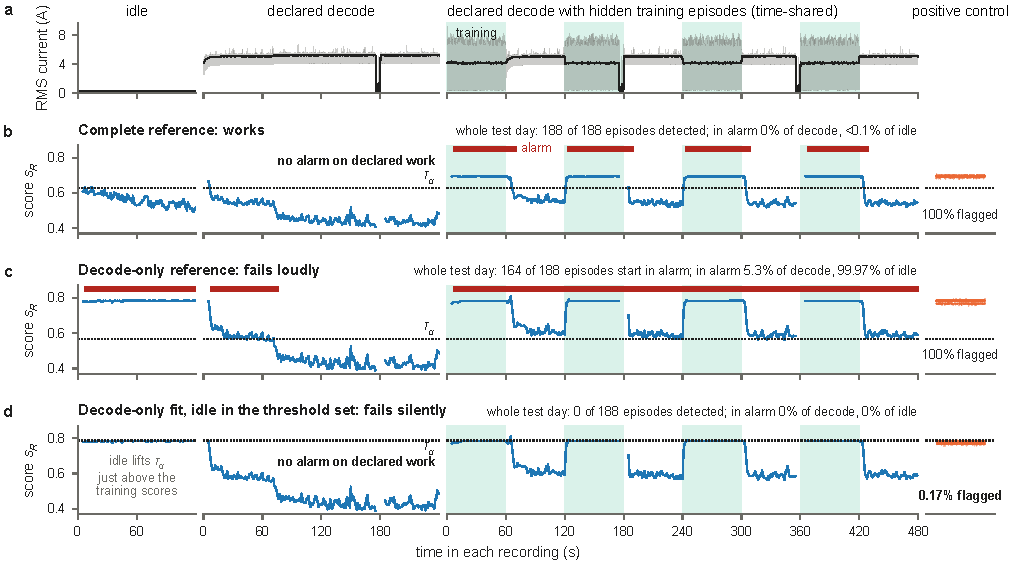
\includegraphics[width=\linewidth]{f8_monitors.pdf}
  \caption{Three configurations of the signature check on the same test-day recordings.
    (a) RMS current in three separate recordings: idle, declared decode, and decode with
    time-shared training episodes (shaded). Line: mean of $e(t)$ per \FeightBin~s; band:
    its 5--95\% range. The dips are unscored seconds. (b)--(d) The score $s_R$, the
    threshold $\tau_\alpha$ (dotted) and the alarm (red bar). (b) The fit holds decode,
    prefill and idle; the threshold set holds decode and idle. (c) Both hold decode only.
    (d) The fit holds decode only; the threshold set holds decode and idle. Right column:
    $s_R$ of honest-training windows from the development data, a positive control.}
  \label{f:f8}
\end{figure*}

The signature check needs no examples of hidden training. With the complete reference, whose fit
holds decode, prefill and idle, $s_R$ at $\tau_\alpha = \TauRone$ detects
$\Ztwo\%$ of co-location windows (development data, one run per training share), and at
least \RoneMinGroup\% of every other evasion group, although it is fitted to
none of them. Its test false-positive rates are \FprRoneDecode\% on decode
and \FprRoneIdle\% on idle.

We also run $s_R$ over the test day as a monitor (\cref{s:monitor}; \cref{f:f8}b).
That day embeds \EpTotal{} time-shared training episodes of \EpMinDur{}~s to
\EpMaxDur{}~s inside declared inference. An episode is detected iff an alarm is active
at some time $t \in [t_{\mathrm{s}},\, t_{\mathrm{e}} + \Grace~\mathrm{s}]$, where its
first step starts at $t_{\mathrm{s}}$ and it ends at $t_{\mathrm{e}}$. An episode with
no alarm is missed, even if it is too short to hold a complete step. We leave out
\EpTruncated{} episodes that the recording cuts short. Both $s_R$ and the classifier, $s_C^{\mathrm{dev}}$,
detect all of the other \EpScored. For $s_R$ the median delay from
first step to alarm onset is $D = \EpDelayRone$~s, and even the shortest episodes
(\LminRone~s) have a within-run lower bound on detection above the target level
of \LminLevel. $s_R$ raises no alarm on test-day decode (\cref{t:t2}). These episodes
test time-sharing only; no co-located episode was recorded.

These results do not hinge on $\alpha$ or on the alarm rule. For $\alpha$ from 1\% to 10\%,
$s_R$ detects \RobCoMin\% of co-location windows and all \EpScored{} episodes, with
\RobOnDecAlpha{} false-alarm onsets on test-day decode and at most \RobOnIdleAlpha{} on idle. Under
persistence rules from 2-of-3 to 5-of-5 it still detects all \EpScored{} episodes, with at
most \RobOnDecPers{} onsets on decode and \RobOnIdlePers{} on idle.

\subsection{The check with an incomplete or corrupt reference}\label{s:monitoring}

\begin{figure}[t]
  \centering
  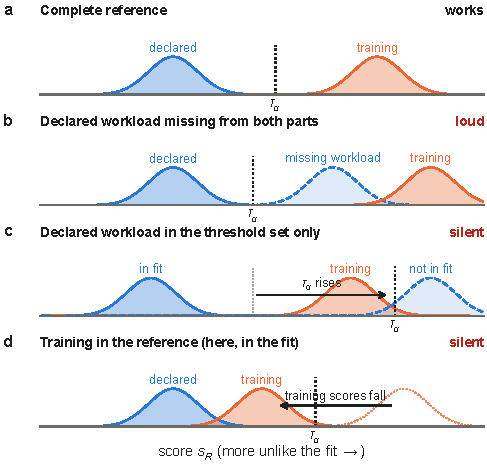
\includegraphics[width=\columnwidth]{f10_reference.pdf}
  \caption{The complete reference (a) and the three changes to it (b--d). Each curve is the distribution of
    the score $s_R$ for one kind of work: declared work (blue) or hidden training
    (orange). The monitor flags every window to the right of the threshold $\tau_\alpha$
    (dotted). (a) The fit and the threshold set hold every declared workload. Training is
    flagged, and declared work is not. (b) One declared workload (dashed) is in neither. It
    scores high and is flagged: a loud failure. (c) The same workload is in the threshold set
    but not in the fit. It still scores high, so $\tau_\alpha$ rises to meet it and
    passes training. Training is no longer flagged: a silent failure. Training in the
    threshold set acts the same way. (d) Training is in the fit. Its scores fall below
    $\tau_\alpha$, so the monitor misses it: also a silent failure. \Cref{t:t7,f:f9} hold the measured cases.}
  \label{f:f10}
\end{figure}

\begin{table*}[tp]
  \centering
  \small
  \resizebox{\textwidth}{!}{% generated by scripts/table_t7.py from (repo_commit of each source):
% h2 41b1fed, r1_scores 53f9463, episodes c574166, false_alarms 1fbe999, heldout dcd87a8, t4 1658809, manifest 018c3a2
% cell sources:
%   full: fit r1_scores.fit_runs.r1; tau set r1_scores.calibration_runs; co-location h2.headline.Z_r1.detection; episodes episodes.detectors.r1.counts; onsets false_alarms.backgrounds.{declared inference,idle}.r1.onsets
%   prefill held out: fit heldout.fit_runs minus panel-serving-prefill; tau set heldout.calibration_runs; flagged heldout.results[family=iforest,variant=R1,alpha=0.05].check4.per_run.panel-serving-prefill.fp_rate; co-location, episodes, onsets: none
%   decode only, decode: fit t4.misspecified_declaration.fit_runs; tau set t4.misspecified_declaration.calibration_runs.declared; co-location t4.misspecified_declaration.declared.h2.r1.co-location.pooled; episodes t4.misspecified_declaration.declared.h3.r1.episodes.counts; flagged t4.misspecified_declaration.declared.dev_stress_fpr; onsets t4.misspecified_declaration.declared.h3.r1.false_alarms.{declared inference,idle}.onsets
%   decode only, decode + idle: fit t4.misspecified_declaration.fit_runs; tau set t4.misspecified_declaration.calibration_runs.pooled; co-location t4.misspecified_declaration.pooled.h2.r1.co-location.pooled; episodes t4.misspecified_declaration.pooled.h3.r1.episodes.counts; flagged t4.misspecified_declaration.pooled.dev_stress_fpr; onsets t4.misspecified_declaration.pooled.h3.r1.false_alarms.{declared inference,idle}.onsets
\begin{tabular}{lllrrlrl}
\toprule
reference & unlike the fit & in $\tau$ set & co-location (\%) & episodes & unlike-fit work flagged (\%) & onsets dec.\ / idle & failure \\
\midrule
complete reference & -- & -- & 100.0 & 0 of 188 missed & -- & 0 / 1 & none \\
prefill held out of the fit & prefill & none & -- & -- & prefill 100.0 & -- & loud \\
decode-only fit, decode threshold set & prefill, idle & none & 100.0 & 164 of 188 start in alarm & prefill 100.0, idle 100.0 & 2 / 4 & loud \\
decode-only fit, decode + idle threshold set & prefill, idle & idle & 0.0 & 188 of 188 missed & prefill 0.0, idle -- & 0 / 0 & silent \\
\bottomrule
\end{tabular}
}
  \caption{The signature check under four references, one per row. ``Unlike the
    fit'': declared work that is not in the fit. ``In $\tau$ set'':
    the part of it that is in the threshold set. Co-location: windows detected at
    $\tau_\alpha$. Episodes: the \EpScored{} scored episodes of the test day; ``start in
    alarm'' means that an alarm is already on when the episode starts (\cref{a:impl}).
    Flagged: windows of the unlike-fit work above $\tau_\alpha$. Onsets: alarm onsets on
    test-day decode and idle.}
  \label{t:t7}
\end{table*}

\begin{figure}[t]
  \centering
  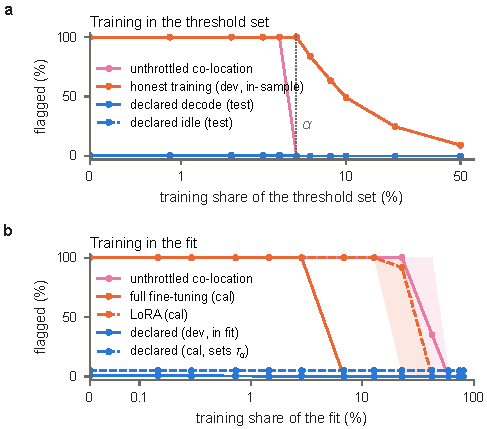
\includegraphics[width=\columnwidth]{f9_contamination.pdf}
  \caption{Training in the reference blinds $s_R$. (a) Honest-training windows added to the threshold set, with the
    fit unchanged and $\alpha = \AlphaPct\%$. The unthrottled run drops to zero near a
    training share of $\alpha$. Honest training is in-sample, since the added windows
    come from its pool. Test decode and idle are flagged less as $\tau_\alpha$ rises.
    (b) Honest-training windows added to the fit, with the threshold set unchanged:
    median over \EfourNDraws{} draws, band from the lowest to the highest draw. Full
    fine-tuning and LoRA are calibration-day runs, outside every fit. The development
    declared windows are in every fit (in-sample). The calibration declared windows set
    $\tau_\alpha$, so their rate stays near $\alpha$ by construction.}
  \label{f:f9}
\end{figure}

The reference is where the signature check can be attacked by an adversarial operator. It is recorded on the
operator's chips, so an operator can try to corrupt it, and even a reference recorded in good
faith can erroneously leave out a declared workload.\footnote{For example, the operator
declares decode, prefill and idle, but the inspectors record only decode. Nobody cheats,
yet the reference is incomplete.} The reference has two parts: the fit, and the threshold set
that fixes $\tau_\alpha$. In \cref{s:works} the fit holds every declared workload, and
the threshold set holds decode and idle.

Here we change the reference in three ways (\cref{f:f10}b--d). Each
change makes the check fail, and each failure is one of two kinds. A \emph{loud} failure
raises alarms on declared work, so the verifier sees that the reference is wrong. A
\emph{silent} failure misses hidden training and raises no alarm on declared work, so
the verifier sees nothing.

\textbf{A declared workload missing from both parts: loud} (\cref{f:f10}b,
\cref{t:t7}). Work that is in neither the fit nor the threshold set raises alarms.
Prefill held out of both is one case (\cref{s:declaration}). A decode-only reference,
with decode alone in the threshold set, is another (\cref{f:f8}c). It detects
\TfourMisCoDeclared\% of co-location, but it is also in alarm for \TfourIdleADecode\% of
test-day idle. A monitor that is almost always in alarm on declared idle is useless, but
it fails loudly. Its alarms show the verifier that it is failing.

\textbf{A declared workload in the threshold set only: silent} (\cref{f:f10}c,
\cref{t:t7}). Keep the decode-only fit, and add idle to its threshold set. The threshold set
now holds decode and idle, which is our default. Idle is now in the threshold set
but not in the fit. It scores high
and lifts $\tau_\alpha$ to \TauDecOnlyPooled{} (\cref{f:f8}d; \cref{f:f7} shows the
scores). The monitor then detects \TfourMisCoPooled\% of co-location and misses all
\EpScored{} episodes. It raises no alarm on test-day decode, just as the complete reference
does. We see that this monitor then fails silently; it does not alert on hidden training, and the verifier has no way to know that it is failing. Prefill is also missing from this fit. Accordingly, with decode alone in the threshold set every prefill window is flagged (\cref{t:t7}). However $\tau_\alpha$ now sits above the prefill scores, and so \DecOnlyPrefillPooled\% of prefill windows are flagged. That is, a missing workload raises alarms only if nothing else
has raised the threshold.

A verifier can expose the silent monitor with a positive control. It gives the monitor
work that it knows to be training, and checks that the monitor flags it. The working
monitor flags \RoneHonestFull\% of development honest training. The silent monitor flags
\TfourPosCtrl\% (\cref{f:f8}, right column).

\textbf{Training in the reference: silent} (\cref{f:f10}c--d, \cref{f:f9}). An operator can
also corrupt the reference, by running training while it is recorded. We test this by
adding windows of training that runs alone on the GPU (honest training,
\cref{s:corpus}) to each part of the reference in turn (\cref{a:reference}). In both cases the monitor comes to miss hidden training, and it
raises no alarm on declared work.

\emph{Training in the threshold set raises $\tau_\alpha$} (\cref{f:f10}c). It takes little training. $\tau_\alpha$ is the $(1-\alpha)$ quantile of the
threshold set (\cref{e:tau}), so once training makes up a fraction $\alpha$ of that set,
$\tau_\alpha$ sits among the training scores. At
$\alpha = \AlphaPct\%$, \EthreeKFive{} windows added to the \EthreeCalWindows{}
calibration windows take detection of the unthrottled run to zero (\cref{f:f9}a). The
higher $\tau_\alpha$ flags declared work less, not more, so the failure is silent. A
positive control of honest training does not expose it, because at that share honest
training is still flagged at $\ge \EthreeHonestMin\%$.

\emph{Training in the fit lowers the scores of training} (\cref{f:f10}d). The fit learns
training as if it were declared work. How much training this takes depends on its kind.
With training at \EfourShareHonest\% of the fit, a full fine-tuning run outside the fit
is flagged at \EfourFullCal\%. The unthrottled run holds longer. Its median detection
reaches \EfourGoneDet\% at a share of \EfourShareGone\% (\cref{f:f9}b). The declared
windows of the fit are flagged at \EfourDeclZero\% with a clean fit, and less as training
is added, so again no alarm shows the failure. This last result is in-sample, because we did not
score held-out declared work under these fits.

\subsection{The open questions}\label{s:declaration}

A verifier who adopts the signature check must still settle four questions
raised by \citet{scher2025} (\cref{s:intro}). Does the signature stay stable
over time? How often will the check raise an alarm? How finely must workloads
be defined? And is the signature specific enough to separate declared work from
hidden work? We answer each in turn from the corpus of \cref{s:corpus}.

\paragraph{Stability over time.} The signature of decode stayed stable over the five days of recording. We recorded
decode in \DecodeRuns{} runs over \DecodeSessions{} sessions, each on a different day.
Three runs are in the reference of $s_R$, two in its fit and one in its threshold set.
Across all \DecodeRuns{} runs, $s_R$ flags
\DecodeFlagged{} of \DecodeWindows{} windows at $\tau_\alpha$, and each flagged window
is the first window of its run. On the two test-day runs, which are outside the reference, its false-positive rate is
\FprRoneDecode\%. Idle was less stable. $s_R$ flags \RoneCalIdle\% of calibration
idle, but only \FprRoneIdle\% of test idle, recorded one day earlier. Because
calibration idle scores above decode, it sets $\tau_\alpha$, and the false-positive rate on test
decode stays well below $\alpha = \AlphaPct\%$.

A reference recorded on a single day does not carry over to other days. In an exploratory check, we
fitted a reference to \SessRefWindows{} windows spread over about four minutes of one
decode run, and repeated this for each of \SessRuns{} runs, one per day. Averaged over
the three runs, this reference flags \SessOther\% of decode from the other days,
against \SessSame\% of the rest of its own run. The two runs recorded to one protocol,
two days apart, give \SessPair\% each way. This reference is not directly comparable to the reference of $s_R$ because it is shorter and flags by a leave-one-out rule rather than $\tau_\alpha$. Nevertheless, this check suggests that the reference should be recorded over several sessions, as the reference of $s_R$ is.

\paragraph{Alarm frequency.} The alarm rate sets how often inspectors must investigate.
On the test day, declared inference is decode only, and the
monitors (\cref{s:monitor}) watch $E = \ExpDecodeH$~h of it (\cref{t:t2}):
\begin{itemize}
  \item $s_R$ raises no alarm: $F = \FRoneDecode$~h$^{-1}$ (95\% upper bound
        \FupRoneDecode~h$^{-1}$), $A = \ARoneDecode$;
  \item the classifier, $s_C^{\mathrm{dev}}$, raises $F = \FClfDecode$~h$^{-1}$ (upper bound
        \FupClfDecode~h$^{-1}$), $A = \AClfDecode$.
\end{itemize}
This exposure is short, so these rates bound the alarm rate only loosely. On idle
($E = \ExpIdleH$~h), both monitors stay near zero.

\begin{table}[tp]
  \centering
  \footnotesize
  % generated by scripts/table_t2.py from results/monitor/false_alarms.json (repo_commit 1fbe999)
% 3-of-5 monitor on 1 s-hop test windows; upper bound: exact Poisson model;
% A interval: approximate onset-block bootstrap (under-covers)
\setlength{\tabcolsep}{3pt}
\begin{tabular}{@{}lrrrr@{}}
\toprule
Detector & onsets & $F$ (/h) & upper (/h) & $A$ (\%) \\
\midrule
\multicolumn{5}{@{}l}{\emph{declared decode}, $E = 0.475$ h} \\
\quad $s_R$ & 0 & 0.0 & 6.3 & 0.0 [0.0, 0.0] \\
\quad $s_C^{\mathrm{dev}}$ & 3 & 6.3 & 16.3 & 1.0 [0.0, 2.0] \\
\midrule
\multicolumn{5}{@{}l}{\emph{idle}, $E = 8.350$ h} \\
\quad $s_R$ & 1 & 0.1 & 0.6 & 0.0 [0.0, 0.1] \\
\quad $s_C^{\mathrm{dev}}$ & 0 & 0.0 & 0.4 & 0.0 [0.0, 0.0] \\
\midrule
\multicolumn{5}{@{}l}{\emph{non-AI busy}, $E = 0.950$ h} \\
\quad $s_R$ & 4 & 4.2 & 9.6 & 99.8 [99.6, 99.9] \\
\quad $s_C^{\mathrm{dev}}$ & 0 & 0.0 & 3.2 & 0.0 [0.0, 0.0] \\
\bottomrule
\end{tabular}

  \caption{False alarms on the test day, per background, with exposure $E$.
    ``upper'': the 95\% upper bound on $F$, which assumes Poisson onsets. Overlapping
    windows make onsets correlated, so this bound is approximate. The intervals on $A$
    come from a block bootstrap (\cref{a:impl}). The test day holds no declared prefill. Non-AI work is undeclared, so $s_R$ is correct to alarm
    on it.}
  \label{t:t2}
\end{table}

\paragraph{Granularity.} The reference must hold each declared workload. When declared prefill
is left out of the reference of $s_R$, $s_R$ flags \RonePrefillHoldout\% of it (one
development run). This is expected, because prefill is limited by compute and decode
by memory bandwidth, so the two load the GPU differently. With prefill
in the fit, $s_R$ flags \PrefillInFitFlagged{} of \PrefillInFitN{} prefill windows.
This rate is in-sample, because neither the calibration day nor the test day holds
prefill. One detector, fitted to decode, prefill and idle together, can therefore
accept all three. The verifier must record every declared workload, but does not
need a separate detector for each. A workload that is in the
threshold set but not in the fit instead raises the threshold (\cref{s:monitoring}).

\paragraph{Specificity.} The signature is specific, but by a thin margin. Under the complete reference, declared
windows score from \DeclBandLo{} to \DeclBandHi{} on $s_R$, and co-location, honest
training and non-AI windows from \HidBandLo{} to \HidBandHi{} (\cref{f:f7}). The two
bands overlap only at the first window of each decode run. The hidden run that comes
closest to declared work is the unthrottled co-location run. Its lowest score,
\RoneUnpacedMin, is \RoneMargin{} above \TauRoneHi, the upper end of the 95\% interval
of $\tau_\alpha$ under a bootstrap of the two calibration runs. With two runs, that end
is the threshold that calibration idle alone would set. The signature check also
does not fully separate this run from declared decode. Its AUC is \RoneAucDecode, and
\RoneDecodeAboveMin\% of test decode windows score above the run's lowest score.

\subsection{Against the default approach}\label{s:missed}

A classifier, like the signature check, works only if its fit covers the declared work.
\Cref{t:t6} sets $s_R$ beside the three classifier fits. It lists what each detector
learns from, its detection of the unthrottled co-location run at $\tau_\alpha$, and its
false-positive rate on test decode.

\begin{table*}[!tp]
  \centering
  \small
  % generated by scripts/table_t6.py from (repo_commit of each source):
% operating_point.json 1d2e0a2, h2.json 41b1fed, r1_scores.json 53f9463,
% windows/manifest.json 018c3a2, replication/t3.json (amodo 73ffebe)
\begin{tabular}{lccccrrl}
\toprule
 & \multicolumn{4}{c}{learns from} & & & \\
\cmidrule(lr){2-5}
detector & declared & honest training & evasions & non-AI & $d_{\mathrm{unthrottled}}(\tau_\alpha)$ & FPR decode & alarm means \\
\midrule
replica & pub. & pub. & -- & pub. & 0.6\% & 0.0\% & training \\
no-evasion fit & \checkmark & \checkmark & -- & \checkmark & 100.0\% & 5.3\% & training \\
$s_C^{\mathrm{dev}}$ & \checkmark & \checkmark & \checkmark & \checkmark & 100.0\% & 1.5\% & training \\
$s_R$ & \checkmark & -- & -- & -- & 100.0\% & 0.6\% & undeclared \\
\bottomrule
\end{tabular}

  \caption{The data each detector learns from, its detection of the unthrottled run at
    $\tau_\alpha$, and its false-positive rate on test decode. ``pub.'': traces recorded
    on the same GPU and probe to the published design, not among the \NCaptures{}
    runs of \cref{s:corpus}. An alarm of $s_R$ means ``undeclared''; an alarm of a
    classifier means ``training''. The rows for the replica and the no-evasion fit are
    exploratory.}
  \label{t:t6}
\end{table*}

At its $\tau_\alpha$, the classifier, $s_C^{\mathrm{dev}}$, does nearly as well as $s_R$.
It detects $\Xprime\%$ of co-location, and every window of every other group except
jitter, where its weakest run is detected at \ClfJitterWorst\%. It stands for the
default approach because it learns from examples of training. But it is fitted on the
monitored GPU, declared work included, as the signature check is, so it needs no
transfer between chips. It is therefore the most favourable case of the default
approach. Even without evasion examples, as in the no-evasion fit, a classifier
needs examples of honest training, whereas $s_R$ needs only recordings of the declared
work.

The threshold of $s_C^{\mathrm{dev}}$ is also fragile. The classifier scores
\FracCalZero\% of calibration declared windows exactly zero, so
$\tau_\alpha = \TauClf$. It then flags any window that stage one calls AI and that even
one of its \ForestTrees{} stage-two trees votes as training. Small changes in declared
work could therefore shift its flags.

A classifier gives no guarantee on a declared workload that its fit has not seen. The
replica, fitted to traces recorded to the published design, detects only
\XzeroPrime\% of the unthrottled run at its $\tau_\alpha$, and flags \RepPrefill\% of
development prefill. $s_C^{\mathrm{dev}}$, which has development prefill in its fit,
flags \ClfDevPrefill\% of it. \citet{gargiulo2026} publish two forests fitted to their
own corpus: a genuine forest, fitted to their training, inference and non-AI traces,
and a hardened forest, which adds their adversarial traces. The two disagree on our
windows (\cref{t:t5}). At their default threshold of \DefaultDecision, the hardened
forest catches all three co-location runs, but it flags \GkHardPrefill\% of declared
prefill windows as training. The genuine forest flags only \GkGenPrefill\% of prefill,
but it misses the unthrottled run ($\GkGenMiss\%$). Nothing in either fit tells the
verifier which outcome to expect. The replica's traces differ from ours in workload
design and session, so its results do not rank the signature check against the default
approach.

\section{Discussion}\label{s:discussion}

The signature check worked when its reference held every declared workload. With no
example of hidden training in its fit, $s_R$ flagged every hidden-training group, and it
raised no alarm on test-day decode (\cref{s:works}). When the reference missed a declared
workload, the check failed in one of two ways (\cref{s:monitoring}). A workload missing
from both parts of the reference kept the monitor in alarm almost continuously while it
ran. This failure was loud, so the verifier could see that something was wrong. A workload in
the threshold set but not in the fit raised $\tau_\alpha$ and blinded the monitor. That
monitor raised no more alarms on declared work than the working one, so the failure was
silent. Such a workload could also mask a loud failure. Training in the reference also blinded the
monitor. So a quiet monitor is no evidence of a working one. The signature check needs no examples of hidden
training in its fit, but the verifier still needs them as positive controls, to test that
the monitor works.

\paragraph{Acquiring a reference and auditing the monitor.} The signature check is only as good as
its reference. The reference is recorded on the monitored chip, where the operator
controls the work. The verifier must therefore control how it is recorded.
\begin{itemize}
  \item \emph{Witness it.} Our reference recordings are our own honest runs. A real
        verifier needs recordings during which the operator cannot train. Both parts of
        the reference are targets. Training at a share of about $\alpha$ in the threshold
        set takes detection of the unthrottled run to zero, and full fine-tuning at
        \EfourShareHonest\% of the fit hides full fine-tuning (\cref{s:monitoring}).
  \item \emph{Span sessions.} A reference from one session flags \SessOther\% of decode
        from the other days (\cref{s:declaration}).
  \item \emph{Test with held-out declared workloads, not only held-out attacks.} A
        declared workload missing from the reference raises alarms
        (\cref{s:declaration}), unless a workload in the threshold set but not in the
        fit masks it (\cref{s:monitoring}).
  \item \emph{Audit the monitor with positive controls that sit close to the
        reference.} The silent monitor flags \TfourPosCtrl\% of honest training, so one
        control run exposes it. But a monitor that flags a control can still miss other hidden work. At the share
        of training in the threshold set that hides the unthrottled run, honest training
        is still flagged (\cref{s:monitoring}). Honest training sits far from the
        reference, so it cannot expose a raised threshold. A control must sit as close
        to the reference as the hidden work it represents.
\end{itemize}
Anomaly detection is hard when normal behaviour is open-ended \citep{sommer2010}. An
agreement can close it, by requiring the operator to declare every workload, so that
anything else is an anomaly by rule. The reference then plays the role of the template in warhead verification, where
the hard problem is to show that the template item is authentic \citep{yan2015}. A
classifier fitted elsewhere, such as the hardened forest of \citet{gargiulo2026}, might
screen recordings offered as declared work, but that forest also flags \GkHardPrefill\%
of our declared prefill (\cref{s:missed}).

\paragraph{What an alarm means.} An alarm from $s_R$ says only that the GPU ran work
unlike its declaration. $s_R$ asks ``is this declared work?'', not ``is this
training?''. Its score does not rank the work it flags, because co-location, honest
training and non-AI work share one band (\cref{f:f7}). As a monitor it is in alarm for a fraction
\ARoneBusy{} of the time on undeclared non-AI work, where the classifier, $s_C^{\mathrm{dev}}$, stays silent
(\cref{t:t2}). Nor does an alarm show that a model was trained.
% results/ceiling/s2.json: tests.r1.primary, rate_a = rate_b = 1.0
The signature check flags every window of a run that discards every update, as it does
for training that applies its updates. An alarm therefore works like an anomaly under
nuclear safeguards~\citep[\S\S 11.24--11.26]{iaea2022glossary}. It opens an inquiry, in
which the operator explains the departure or the verifier inspects. No conclusion is drawn until the
operator has had the chance to explain~\citep[Art.~4.d]{iaea1997ap}. The false-alarm rate
per hour sets how often the verifier must inquire, and so the cost of the regime
(\cref{s:declaration}).

\paragraph{Limits.}
\begin{itemize}
  \item \emph{Scale.} We use one model and one GPU, with one run per co-location share,
        and we do not test one probe on several GPUs at once. Co-location is development
        data from one session. The evasions did not adapt to the detector. Our corpus
        has no diluted LoRA. The scale, the chip activity measured and the threat model
        of \citet{scher2025} are wider than ours.
  \item \emph{Code access.} \citet{scher2025} rely on temporary code access to
        label the recordings, and to review the code after an alarm. We test neither.
        Our reference recordings are our own honest runs, and we test only whether the
        signal departs from them.
  \item \emph{Hardware.} We test no transfer between chips. Every detector we fit,
        the classifiers included, is fitted and scored on the GPU we monitor, and the
        published forests of \citet{gargiulo2026} come from the same GPU model and probe
        model. The default approach must transfer in practice, so our comparison
        favours it. The signature check needs no transfer, but its reference must hold
        across sessions.
  \item \emph{Exposure.} The test day holds no prefill and only \ExpDecodeH~h of
        declared decode, so the false-alarm bounds are loose, and declared prefill is a
        risk we could not measure on held-out data.
  \item \emph{Amplitude.} The unthrottled run draws a median AC RMS current of
        \AcRmsUnpaced~A, against \AcRmsDecode~A for development decode, and the per-run interquartile ranges do not overlap. So
        amplitude alone would separate this run from decode, and the run is not a hard
        case for a detector that uses amplitude. Our features are amplitude-free and do
        not use it. A harder test would match the amplitude of declared decode.
  \item \emph{Design.} Our results depend on our split of the reference into a fit and
        a threshold set (\cref{t:t7}), whereas \citet{scher2025} specify one baseline.
        One short calibration run each of decode and idle sets $\tau_\alpha$
        (\cref{t:corpus}). That idle run is unlike test idle, since $s_R$ flags
        \RoneCalIdle\% of it but only \FprRoneIdle\% of test idle. Resampling whole calibration runs moves
        $\tau_\alpha$ over [\TauRoneLo, \TauRoneHi].
  \item \emph{Training data in view.} The signature check uses no training or evasion
        examples in its reference, but three earlier choices drew on them. Its features
        come from \citet{gargiulo2026}, who chose them to separate training from
        inference. When we chose its design, we required each candidate to flag at least
        \PosControlMin\% of honest-training windows from an unseen session. Every
        candidate passed, so this requirement did not decide the choice. We also measured its detection on development data
        before we scored any test data. Only its test false-positive rates and the monitor
        results are held out.
  \item \emph{Contamination.} We test contamination only in the exploratory checks of
        \cref{s:monitoring}, with training drawn from our own runs.
  \item \emph{Measurement chain.} Our measurement chain and that of \citet{gargiulo2026}
        differ in sample rate, filtering and feature set (\cref{a:gk}).
\end{itemize}


\bibliography{references}
\bibliographystyle{icml2026}

\appendix
\crefalias{section}{appendix}
% Appendix tables and figures are numbered A1, A2, ... so a main-text citation shows where they are.
\setcounter{table}{0}
\renewcommand{\thetable}{A\arabic{table}}
\renewcommand{\theHtable}{A\arabic{table}}
\setcounter{figure}{0}
\renewcommand{\thefigure}{A\arabic{figure}}
\renewcommand{\theHfigure}{A\arabic{figure}}
\crefname{appendix}{Appendix}{Appendices}
\Crefname{appendix}{Appendix}{Appendices}
\onecolumn
\section{Implementation}\label{a:impl}

\paragraph{Channel.} A \Digitiser{} oscilloscope digitises the probe at \DigBits{}~bits
and streams the raw samples at \Fs{}~S/s. No filter precedes the converter, so current
variance above the Nyquist frequency folds into the band. We bound it from bursts
recorded at \BurstRate{}~MS/s, assuming no rejection. Under training the folded
variance is at most \AliasTrainPct\% of the in-band variance. Under idle, where the
current is small, it is at most \AliasIdleX{} times the in-band variance. At this bound,
both the raw-spectrum and the envelope features of idle windows would mostly describe
folded variance. Idle windows help set each detector's $\tau_\alpha$ and fit $s_R$, so a
different digitiser or an anti-alias filter could move them; we did not test this. The
low rate costs little signal. In the same bursts, \ChainBelowBand\% of a training trace's variance lies below
\ChainBandKhz{}~kHz, and the envelope at our rate matches one sampled ten times faster
to within \ChainEnvPct\%.

\paragraph{Corpus.} \Cref{t:corpus} counts runs, hours and windows per workload and
split.

\begin{table}[!htbp]
  \centering
  \small
  % generated by scripts/table_corpus.py from results/windows/manifest.json (repo_commit 018c3a2, corpus_commit 73ffebe)
% runs, scored hours and 5 s-hop windows per workload and split
\begin{tabular}{lrrrrrrrrr}
\toprule
 & \multicolumn{3}{c}{$\mathcal{D}_{\mathrm{dev}}$} & \multicolumn{3}{c}{$\mathcal{D}_{\mathrm{test}}$} & \multicolumn{3}{c}{$\mathcal{D}_{\mathrm{cal}}$} \\
\cmidrule(lr){2-4}\cmidrule(lr){5-7}\cmidrule(lr){8-10}
Workload & runs & h & windows & runs & h & windows & runs & h & windows \\
\midrule
honest training & 14 & 4.06 & 2905 & 4 & 0.95 & 680 & 2 & 0.48 & 340 \\
time-sharing & 3 & 0.71 & 510 & 7 & 2.22 & 1586 & -- & -- & -- \\
co-location & 3 & 0.72 & 510 & -- & -- & -- & -- & -- & -- \\
jitter & 4 & 0.95 & 678 & -- & -- & -- & -- & -- & -- \\
padding & 1 & 0.24 & 170 & -- & -- & -- & -- & -- & -- \\
power cap & 2 & 0.48 & 340 & -- & -- & -- & -- & -- & -- \\
declared decode & 2 & 0.48 & 340 & 2 & 0.48 & 340 & 1 & 0.24 & 170 \\
declared prefill & 1 & 0.24 & 170 & -- & -- & -- & -- & -- & -- \\
declared idle & 1 & 0.24 & 170 & 4 & 8.35 & 5994 & 1 & 0.24 & 170 \\
non-AI work & 4 & 0.95 & 681 & 4 & 0.95 & 680 & 2 & 0.48 & 340 \\
\midrule
total & 35 & 9.06 & 6474 & 21 & 12.94 & 9280 & 6 & 1.43 & 1020 \\
\bottomrule
\end{tabular}

  \caption{The corpus per workload and split: runs, scored hours and windows at the
    window-level hop. Time-sharing on the test day is the embedded episodes of
    \cref{s:works}.}
  \label{t:corpus}
\end{table}

\paragraph{Detectors.} The classifier's two stages are random forests and the
signature check is an isolation forest, all from scikit-learn with \ForestTrees{} trees,
default settings otherwise and a fixed seed.

\paragraph{Intervals.} For one run, a circular block bootstrap resamples blocks of
\BootBlock{} consecutive windows (\BootBlockS~s), \NBoot{} times
(\NBootBound{} for the episode lower bounds and the equivalence test). For two runs it
resamples within each run and pools. For three or more it resamples runs. Thresholds
stay fixed in every resample. On the monitor, the upper bound on $F$ assumes Poisson
onsets; the interval on $A$ resamples blocks of \OnsetBlockMin~min. An episode lower bound
is the smaller of a one-sided Clopper--Pearson bound and a block bootstrap over blocks
of \EpBlock{} consecutive episodes.

\paragraph{Episodes.} An episode that starts while an alarm is active counts as
detected only where the run's flag rate on gap windows, which hold no training, is at
most \GapGuard; we call this the gap guard. A run whose gaps hold no whole window takes the pooled gap flag rate
of the other runs. Otherwise only new onsets count, and the result is marked
onset-only. The delay $D$ is taken over episodes that raise a new alarm.
Under the complete reference, \EpPreRone{} of the \EpScored{} scored episodes start in alarm, and all are
credited (\cref{t:t7}).

\paragraph{Data and code.} The corpus is archived on Zenodo
\citep{kimpson2026corpus}. The analysis code, every committed result, and the scripts
that make every figure, table and number in this paper are at
\url{https://github.com/tomkimpson/verifying-declared-ai-workloads}. The window
features are not stored there; \texttt{scripts/make\_windows.py} regenerates them from
the archive. Every result
was computed against corpus commit \texttt{\CorpusCommit}.

\FloatBarrier
\section{The reference changes in detail}\label{a:reference}

\paragraph{Scores.} \Cref{f:f7} shows the per-window scores behind the complete
reference and the decode-only fit of \cref{t:t7}.

\begin{figure}[!htbp]
  \centering
  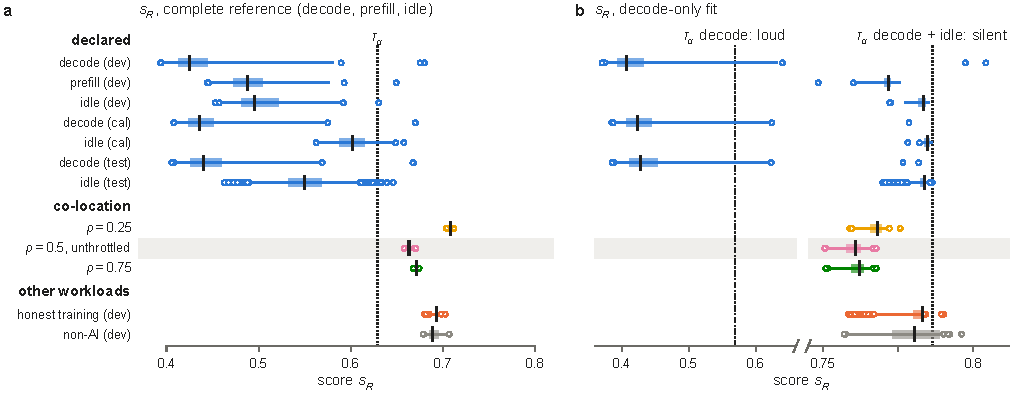
\includegraphics[width=\linewidth]{f7_r1.pdf}
  \caption{How $s_R$ scores each workload. Each row shows the per-window scores of one
    workload and split. Black ticks mark medians, bars the 25--75\% range and whiskers
    the 1--99\% range; circles are single windows beyond the whiskers. Windows to the right
    of $\tau_\alpha$ (dotted) are flagged. (a) The complete reference, with
    $\tau_\alpha = \TauRone$. It flags every co-location, honest-training and non-AI
    window. The shaded unthrottled run is the co-location run closest to $\tau_\alpha$; a
    few decode windows score above it (AUC \RoneAucDecode). (b) The decode-only fit
    (\cref{t:t7}), on a score axis broken at the slashes and widened beyond them. Prefill
    and idle are outside this fit, and idle now scores high. With idle in the threshold
    set, $\tau_\alpha = \TauDecOnlyPooled$ and no co-location window is flagged. With
    decode alone in it, $\tau_\alpha = \TauDecOnlyDecode$ and every co-location window
    and every idle window is flagged. Each threshold is labelled by its failure, as in
    \cref{t:t7}.}
  \label{f:f7}
\end{figure}

\paragraph{Training in the threshold set.} We add $k$ honest-training windows to the
\EthreeCalWindows{} calibration windows, with the fit unchanged. Detection of the
unthrottled run falls to zero at $k = \EthreeKOne$ to \EthreeKTen{} for $\alpha$
from 1\% to 10\%, and at $k = \EthreeKFive$ for $\alpha = \AlphaPct\%$. At that $k$, honest
training is still flagged at $\ge \EthreeHonestMin\%$; it falls as $k$ grows further
(\cref{f:f9}a).

\paragraph{Training in the fit.} We add $k$ development honest-training windows, drawn at
random, to the \EfourNDeclared{} declared windows of the fit, with the threshold set
unchanged. At $k = \EfourKHonest$ (\EfourShareHonest\% of the fit), the calibration-day
full fine-tuning run, which is outside every fit, is flagged at \EfourFullCal\%, while
LoRA stays at \EfourLoraCal\%. The median detection of the unthrottled run is
\EfourHalfDet\% at $k = \EfourKHalf$ and \EfourGoneDet\% at $k = \EfourKGone$
(\EfourShareGone\% of the fit). The declared windows of the fit are flagged at
\EfourDeclZero\% with a clean fit, and at \EfourDeclEnd\% at the largest $k$ (median over
draws; \cref{f:f9}b). These windows are in every fit, so the rate is in-sample.

\section{The cross-check on the corpus of Gargiulo and Kulp}\label{a:gk}

We fetched their \GkNTraces{} traces \citep{gkdataset} at a pinned revision, checked each file's hash,
and resampled from \GkRate{}~MS/s to \GkDecimated{}~kS/s with an exact rational
resampler and its anti-alias filter. We extracted our \NFeat{} features and fitted
their two forests: genuine, on their training, inference and non-AI traces; hardened,
adding their adversarial traces.

On their own traces, under their grouped five-fold protocol, our measurement chain reaches
macro-$F_1$ \GkOwnFone{} (range \GkOwnFoneLo{} to \GkOwnFoneHi) and accuracy
\GkOwnAcc. They report \GkFone{} and \GkAcc{} with \GkNFeat{} features at the full
rate. We did not reach their accuracy, and scored our windows anyway. Shuffled labels give \GkShuffle. Their traces pass an anti-alias
filter on decimation and ours do not, so features above about \GkAliasKhz{}~kHz differ
between the datasets.

\paragraph{The published hardened forest.}
\citet{gargiulo2026} harden their forest on four evasion strategies of their own. We
scored our windows with both forests (\cref{t:t5}). At their default threshold of
\DefaultDecision, their genuine forest misses the
unthrottled run ($\GkGenMiss\%$). Their hardened forest catches all three
co-location runs, but it also flags \GkHardPrefill\% of declared prefill windows as
training. Their hardening works here. Its cost falls on a declared workload that our
calibration day does not hold.

\begin{table}[!htbp]
  \centering
  \small
  % generated by scripts/table_t5.py from results/gk/t5.json (repo_commit 4494926)
% percent of windows flagged training; co-location over windows with >= 1 complete step
\begin{tabular}{lrr}
\toprule
Our windows & G\&K hardened & G\&K genuine \\
\midrule
honest training ($\geq 80$\%) & 100.0 & 100.0 \\
declared decode & 0.0 & 0.0 \\
declared prefill & 100.0 & 2.4 \\
declared, decode + prefill ($\leq 20$\%) & 16.7 & 0.4 \\
\midrule
co-location, $\rho = 0.25$ & 100.0 & 100.0 \\
co-location, $\rho = 0.5$ & 100.0 & 0.0 \\
co-location, $\rho = 0.75$ & 100.0 & 100.0 \\
\bottomrule
\end{tabular}

  \caption{Forests fitted by the recipe of \citet{gargiulo2026} (G\&K) on their corpus,
    scored on our windows: percent flagged training. The first rows are a
    transfer gate (training $\geq$ \GateTrain\%, declared
    $\leq$ \GateInf\%). Both forests pass. The hardened forest passes the declared
    row only because decode outnumbers prefill. Their chain and ours differ in rate
    and anti-alias filtering, and their own-data check fell short of their reported
    accuracy (\cref{a:gk}).}
  \label{t:t5}
\end{table}

\FloatBarrier

\end{document}
